\section{Dropout}
\label{sec:dropout}

Neural networks, like many other learning algorithms, can suffer from overfitting the data.
A simple technique to avoid overfitting in deep networks is the Dropout.

Dropout is an extremely simple and effective technique recently introduced by Srivastava et al.\ \cite{srivastava2014dropout}.
It consists in randomly turning off perceptrons during the training phase:
at each epoch of training, perceptrons are kept active only with some probability p (a hyperparameter), otherwise they are set to zero.
The process can be see in \cref{fig:dropout}, taken from the original paper.
Dropout is not applied during test and allows to ensemble the different parameters learned by some group of perceptrons during the training.

\begin{figure}[ht]
	\centering
	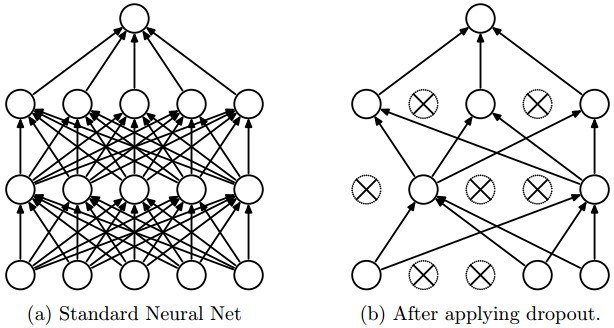
\includegraphics[width=\columnwidth]{figures/dropout}
	\caption{Changes in the neural network after applying Dropout.}
	\label{fig:dropout}
\end{figure}
